\documentclass{article} % For LaTeX2e
\usepackage{nips15submit_e,times}
\usepackage{hyperref}
\usepackage{url}
\usepackage{graphicx}
%\documentstyle[nips14submit_09,times,art10]{article} % For LaTeX 2.09

\title{INCAT : Intelligence-based Cybersecurity Awareness Training}
\author{
Tam n. Nguyen, Lydia Sbityakov, Samantha Scoggins\\
North Carolina State University\\
\texttt{\{tam.nguyen, lesbitya, smscoggi\}@ncsu.edu} \\
}
\newcommand{\fix}{\marginpar{FIX}}
\newcommand{\new}{\marginpar{NEW}}
\nipsfinalcopy % Uncomment for camera-ready version
\begin{document}
\maketitle

\begin{abstract}
  Cybersecurity training should be adaptable to evolving cyber threat landscape, cost effective and integrated well with other enterprise management components. Unfortunately, very few cyber security training platforms can satisfy such requirements. This paper proposes a new novel model for conducting cyber security trainings with three main objectives: (i) trainings should be initiated by emerging relevant threats and delivered first to the most vulnerable members (ii) the process has to be agile (iii) training results must be able to provide actionable intelligence. For the first time, the paper establishes a type system (ontology and associated relationships) that links the domain of cyber-security awareness training with that of cyber threat intelligence. Powered by IBM Watson platform, the proposed method was found to be practical and scalable. Main contributions such as exports of the type system, the manually annotated corpus of 100 threat reports and 127 cyber-security assessment results, the dictionaries for pre-annotation, etc were made publicly available.
\end{abstract}

\section{Introduction}
The threat landscape is constantly changing. Something that was not considered a vulnerability yesterday may now become one \cite{Manadhata2011AnMetric}. Therefore, cyber-security awareness training (CAT) should be adaptable, be cost effective and most important of all, be integrated well with other components such as enterprise risk management, incident management, threat intelligence and so on. Unfortunately and in most cases, CAT is not a strong component in most cyber defense strategy \cite{Jakoubi2009AManagement}.

This lack of emphasis on human training and analysis leads to greater issues with establishing cyber security requirements, cyber incident's impact determination, and the simulation of possible attack scenarios. For example, security requirements tend to be mechanical 1-on-1 mappings from obvious security features and regulatory controls \cite{Cleland-Huang2014HowGratae}. Consequently, there is a very common assumption that most malicious hackers will seek the path of the most devastating exploits. In realities, hackers do not follow a straight line while using only a fraction of available vulnerabilities to deliver attacks \cite{Allodi2017TowardsAssumptions}. A lot of those vulnerabilities deal directly with human errors \cite{Messaoud2017AdvancedChallenges}.

Also, it is found that when evaluating cybersecurity risks, there are fixation on binary events without consideration of fuzzy states in between, and bias toward the point of view of security management (more technical) rather than overall business goals (more human oriented) \cite{Dhillon2011Developer-drivenTrenches} \cite{Bayuk2013SecurityConstruct}. Last but not least, common reported threat metrics can be highly debatable among teams and agencies \footnote{https://bit.ly/1yJcGjC} since numbers cannot describe all possible underlining context. 

This paper proposes InCAT - a new model for conducting cyber security training with a strong focus on drilling deep into the shared contexts among collected cyber awareness training results, cyber threat intelligence reports, and other cyber security related data logs. InCAT stands for "Intelligence-based Cyber Awareness Training" and its feedback loop starts with a threat intelligence feed where the most recent cyber threats will be analyzed by machine learning models to identify the current attack-defense themes. This angle is called "Technical Angle". From the identified themes, quizzes will be sent to users (samples) within a company (population). Machine learning models will analyze users' responses with expected results such as a list of vulnerabilities for which employees are least prepared for. This angle is called "Human Angle". Actionable intelligence can then be derived from analyzing results gathered from both angles.

The main contributions of this paper include: (i) A novel new model for conducting cyber-security awareness training that is highly adaptive to threat landscape (ii) Downloadable type system, dictionaries and human annotated data-sets for further customization and studies, (iii) Exported machine learning models and starter code base for immediate deployment. Background and related works are presented in Section 2. High-level design structure and elaborations on our methodologies are presented in Section 3. Implementation details including links to demos, source codes, sample data and results are presented in Section 4. Self-critical evaluations of this research project will be presented in Section 5 to be followed with plans for future works listed in the Conclusion section.

\section{Backgrounds}
Human is the weakest link in any cyber defense strategy. 78\% of cyber incidents were caused by careless humans \cite{20172017Overview}. The process of cyber awareness training is full of challenges. First, the threat landscape is evolving rapidly with both internal factors (technology changes, business flows changed, etc) and external factors (changes in supply chain, compliance, competitors, enemies, political climates, etc) \cite{Ingalsbe2008ThreatEnd, Manadhata2011AnMetric}. To make things worst, there is no agile cooperation between cyber awareness education and other departments. 

Second, knowledge is not always translated into correct actions. For example, people who know the types of phishing are not completely immune from actual phishing. Training materials are more focused on teaching the knowledge rather rather the skills of applying the knowledge. Consequently, tests are developed to test just the knowledge, in which case learners are well aware that they are being tested and consciously put their guards on. It is very hard to simulate real world scenarios.

Finally, it is challenging to prepare people for potential unknown threats that have not happened yet, not mentioning cyber adversaries are incredibly creative, sometimes state sponsored.

Abawajy \cite{Abawajy2014UserMethods} did a research on user preference of cyber security awareness methods of text-based, video-based and game-based among 60 participants. Even with a "low-tech" appearance, the performance of text-based education is on par with other "fancy" methods. Employees with work deadlines and projects actually prefer light-weight cyber security awareness delivery method that does not get in the way of their main jobs.

Pawlowski \cite{Pawlowski2016SocialDesign} presented a way to map learners' perceptions toward cyber security topics using data analytics.  Especially of interest for high-impact cyber security training is finding out which topics are either high-interest (may affect individuals personally) or low-awareness (security blind spots) for learners.  Additionally, from a management perspective, how learners can be motivated to continue to learn and stay abreast of new threats is also of high importance.  It was discovered that learners have been exposed to several cyber security key terms and concepts, care very much about cyber security topics that may affect them personally, but that they lack awareness of the bigger picture which also includes national cyber infrastructure and cyber terrorism.

Wei \cite{Wei2017IntegratingAssessment} adopts concept mapping (CM) as a tool to enhance the teaching and evaluating of Information System courses. By analyzing the topology of student CMs, instructors can design CM-based tasks, and grade student CMs against a master CM. While it was not explicitly mentioned in the paper, comparing CM is a very interesting way to identify how the concept map of a student can be changed over time, by education and other factors.

Green \cite{Green2018TowardsSchemes} proposed an alternative to regular text-based machine learning approach with heavier emphasis on argument mining. The process involves steps of careful annotation of a selected corpus, building logic rules or relationships based on domain specific knowledge, and finally, inferring arguments. The paper made a case for more sophisticated content analysis method when dealing with complex contents such as biological research papers.

Joshi \cite{Joshi2013ExtractingText} described a strategy of "combining" intelligence gathered from both structured and unstructured texts to form actionable intelligence in the domain of cyber security. The approach relies on a custom ontology for cyber security domain and a "concept extractor" built using various open-source products.

Ferruci \cite{Ferrucci2010BuildingProject} wrote about IBM's billion dollar baby - Watson, and proves that within a large knowledge domain such as Jeopardy's, not only deep learning can understand human languages and response with thoughtful insights, but it can also perform reliably in real time. To sum up the strength and weaknesses of Watson, Deloitte did provide a very good report \cite{DeloitteDevelopment2015DisruptionWatson} in 2015. At the time of this paper, IBM Watson has been deployed commercially in various domains including health care, finance, insurance and so on.

\section{Methodology and Designs}
InCat feedback loop includes 8 main steps as shown in Figure \ref{Figure:IncatDesign}. 

\begin{figure}[h]
  \centering
  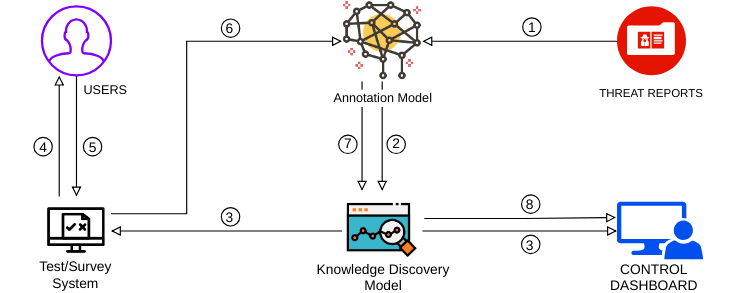
\includegraphics[width=11cm]{images/INCAT-Designs.png}
  \caption{INCAT Design Structure}
  \label{Figure:IncatDesign}
\end{figure}

Threat reports are highly condensed data that relates to cyber threat developments and was prepared by domain experts. Reports will be analyzed by the Annotation Model for identification of key entities and the relationships between them. Newly annotated data will be further analyzed by the Knowledge Discovery Model which will automatically identify newly emerged patterns in cyber threat landscape. The Test/Survey System will construct assessments based on the knowledge components relating to the newly identified patterns and deliver to the users who are most vulnerable. Assessment results will then be returned to the Test/Survey System for initial processing, resulting in reports with scores and users' response texts. Such user assessment reports will be analyzed by the same Annotation Model and the Knowledge Discovery Model. Derived knowledge from threat reports (step 3) and user assessment reports (step 7) are stored in database and be displayed by a Control Dashboard system. Through this dashboard, cyber security analysts may correlate details and derive further actionable intelligence.

\section{Implementation}
\subsection{Data Source and Preprocessing}
The nvd database was already a high quality data set so minimal manipulation of the data was needed for pre-processing. From the 2018 vulnerability json file, CVE-2018, downloaded from https://nvd.nist.gov/vuln/data-feeds on September 19th (The file is continually updated).  We then created two data sets.  For text analysis we extracted the CVE-ID number and description for 8748 records.  The categorical data set consists of all 6851 available 2018 nvd records with a completed base metric 3 (BM3) section.  These features generally correspond to the vulnerability ontology used in the text analysis (see next section) which is based on the NIST17 paper \cite{}: For clustering we extracted the CVE-ID and categorical fields (listed in the table below along with their possible values).  Derivative fields such as baseScore and baseSeverity that are calculated from other fields were eliminated from cluster processing.  We choose to work with the more updated Base Metrics 3.0.   Only the fields of Product and Vendor were sometimes missing and these were imputed to the value of "UNKNOWN" in these cases.  

\subsection{Identifying Attack vectors}
\begin{center}
\begin{tabular}{ |l|l| } \hline
Feature & Values\\\hline
Attack Vector & Network, Adjacent, Local, Physical  \\ 
Attack Complexity & Low, High  \\ 
Privileges Required & None, Low, High  \\ 
User Interaction & None, Required  \\ 
Confidentiality Impact & High, Low, None\\
Integrity Impact & High, Low, None\\
Availability Impact & High, Low, None\\
\hline
\end{tabular}
\end{center}


This relatively small set of features and possible values can have 1,296 different combinations.  However, a simple data query reveals that only 236 combinations were associated with any threats and 74.7\% of the vulnerabilities fall into just 16 unique combinations of features. Finding meaningful clusters in the data would help to focus training on the most prevalent threat vectors and make the most efficient use of resources.  

Clustering was used to determine if there was a natural clustering of features and if certain combinations were never seen or exceedingly common. In addition, the features of product and vendor are also available for many records.  Clustering was performed both with and without the additional fields of product and vendor.

Because the data is purely categorical common algorithms such as k-means are not recommended. \cite{}.  DBScan while helpful for removing outliers is not recommended for data with higher dimensions where Euclidean distance is less effective \cite{}.  
Cluster analysis was performed using python and the k-modes module \cite{https://pypi.org/project/kmodes/} \textit{which defines clusters based on the number of matching categories between data points.}   because this package is readily available and specifically designed to work with categorical data.  

\textit{Describe clusters here.
}
The clustering results serve to inform the annotation and classification process used in 4.2 and in future could provide the underlying framework for the identification and selection of Attack Vectors on an on-going basis.



\subsection{Annotation Model for Classifying Text Data}
Our data sets of descriptions for Threat Reports were extracted from the National Vulnerability Database which can be considered the gold standard of threat reporting and is being used nation wide. In the form of XML or CSV files, datasets can be imported into Annotation Model which is powered by the IBM Watson Knowledge Studio platform \footnote{https://www.ibm.com/watson/services/knowledge-studio/}.

There are three main steps for building the Annotation Model: (i) Building a system type (ii) Building ground truths by manual annotation (iii) Training and evaluating models.

A system type is a domain-specific ontology enriched with relationships. Since the domain is Cyber Security, we decided to rely on another gold standard - the NIST's recommendations for Cyber Vulnerability Description ontology \cite{Booth2016DraftOntology} which was summarized into Figure \ref{Figure:VulOntology}.

\begin{figure}[h]
  \centering
  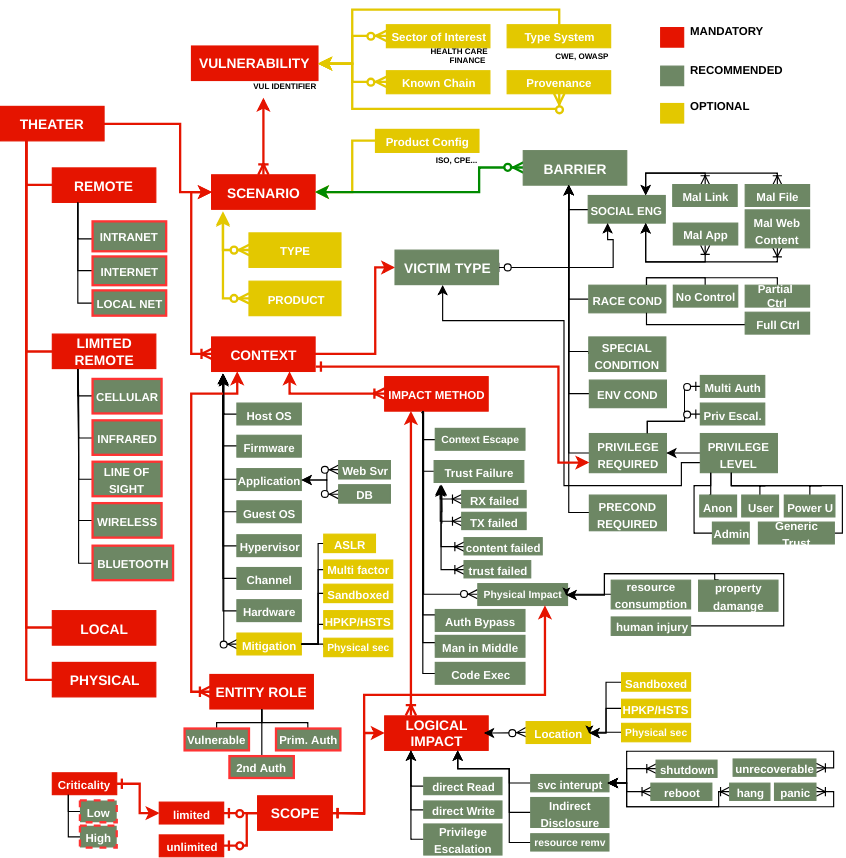
\includegraphics[width=12cm]{images/NISTIR8138.png}
  \caption{Vulnerability Description Ontology}
  \label{Figure:VulOntology}
\end{figure}

It is notable that in real-world scenario, reports will only touch a few "boxes" of this crowded ontology. Therefore, the ontology has to be enriched with relationships that are context-preserving. Such relationships can be described directly by rules or indirectly by type \& sub-type specifications. The novelty of our work comes in the form of our own designed relationship rules, the overloading of the rules and the re-mapped hierarchy of the original NIST's ontology. The detailed description file of our type system (ontology with relationships) can be viewed at our Github repository \footnote{https://github.com/genterist/INCAT-public}. Further elaborations on this type system will be on the final full paper.

In order to build ground truths, we started first with human annotators and manual annotation. Small sets of 50 entries each are extracted from our corpus of 1000 NVD threat reports in 2018. Sets can be specified to have some overlaps in order to support inter-annotation. Team members (except one) will work on their corresponding pre-assigned sets and manually annotate entities together with relationships. At the final step, the one who did not do any manual annotation will go over the results, resolve conflicts and publish annotated entries as ground truths.

On the IBM Watson Knowledge Studio platform, we train and test our models using the manually annotated entries which are separated into training set (70\%), test set(23\%), and blind set(7\%). Training set is used to teach machine the domain specific knowledge through annotated entities and their relationships. Trained model will then perform on test set to produce test set machine results. Upon comparing test set machine results with human annotated results, the accuracy of the model can be defined. Blind set is used to test the system only after several iterations of training and testing. The end result of this process is an annotation model that can be deployed with other models which, in our case, happened to be IBM Knowledge Discovery.

\subsection{Training and Evaluating the Model}
put content here

\section{Conclusion}
InCAT is a new model for conducting cyber security training with three long term goals: (i) training efforts are initiated by emerging relevant threats and delivered first to the most vulnerable groups (ii) each training session must be promptly executed (iii) training results must be able to provide actionable intelligence to be employed by other systems such as enterprise risk management, enterprise threat intelligence, etc.

The project is the first in making an attempt at constructing a type system that allows the inter-connecting of intelligence among cyber-security related domains, including cyber-security awareness training. The project is also the first in designing an intelligence-driven rather than compliance-driven or knowledge-driven process for conducting cyber-security awareness training. Within a very short amount of time, the project was able to provide preliminary results including a manually annotated corpus of 100 threat reports, and 127 cyber-security awareness training assessments; a set of dictionaries for pre-annotation; and an annotation model capable of 66\% entity marking coverage with 75\% accuracy.

Basic research questions were answered and directions for future developments are clear: (1) Deeper research into inter-domain ontology design and upgrade the type system, (2) Significantly extend the words in dictionaries for more comprehensive pre-annotation (3) Integrate Prolog into work flow, allowing it to work in parallel with the machine learning model (4) Extend the corpus with more human annotated contents.

\bibliographystyle{IEEEtran}
\bibliography{IEEEabrv,references.bib}

\end{document}